
%%%%%%%%%%%%%%%%%%
\chapter{Economics of Experiments}
\section{Motivation}
In previous chapters, we have learned that one way to control for many internal validity threats - such as selection bias, omitted variable bias - is an \textbf{ideal randomized controlled experiments}. This is where you categorize some individuals under treatment group and controlled group and run various tests as if you are in a laboratory experiment. While there are some degrees of randomized controlled experiments (not necessarily ideal, in the sense that subjects were not brought to the lab), this is difficult to conduct, due to logistical, financial, and ethical reasons. The alternative is to use a \textbf{quasi-experiment} or \textbf{natural experiments}. This is where there exists an exogenous event (like natural disasters, policy change etc) that affect some groups of the population differently than the others.  To see the impact of the said event, we need to be able to compared the affected group (treatment) and the unaffected group (controlled) across different time periods. \par\medskip

So what is the value in studying experiments? For one thing, they provide a conceptual benchmark for assessing observational studies. In particular, experiment is one of the ways to see how economic theories can be applied in reality. More importantly, unlike surveys, they are free from various internal validity threats. Surveys suffer from selection bias - if people don't respond to surveys anymore and they are different from those who respond, we fail to obtain a representative sample. However, experiments suffer from their own validity threats. 
\begin{mdframed}[backgroundcolor =blue!10]
\textbf{Example of randomized controlled experiments}
\begin{itemize}
\item \textit{What are the barriers to technology adoption?} This is from a research of Prof. Eric Verhoogen of Columbia (with some co-authors)\footnote{\scriptsize{Atkin, D., A. Chaudhry, S. Chaudry, A. K. Khandelwal, E. Verhoogen (2017), Organizational Barriers to Technology Adoption: Evidence from Soccer-Ball Producers in Pakistan, \textit{The Quarterly Journal of Economics}, 132(3): 1101–1164}}. This team of researchers developed a new cutting technology that reduces waste of primary raw material involved in making soccer balls. Initially it gave a random subset of Pakistani producers an access to the technology. The take-up rate was very low, for surprising reasons. Then, they noticed that the employees get paid according to the number of soccer balls made, not taking into account the waste of resources involved. Since the new technology slowed them down initially, employees were reluctant to accept new technology. Then, the team conducted another experiment within the firms that had the access to the technology. Within each firm, one cutter and one printer received a lump-sum payment equivalent to monthly earnings. However, there is a string attached - each worker must be able to use the technology in presence of their owner. As a result, employees accepted the new technology more. \par\medskip
\noindent
\end{itemize}
\textbf{Example of natural experiments}
\begin{itemize}
\item \textit{What are the impacts of prenatal exposure to radioactive fallout?} This is from Prof. Douglas Almond and Prof. Lena Edlund's research\footnote{\scriptsize{D. Almond, L. Edlund, M. Palme (2009), Chernobyl's Subclinical Legacy: Prenatal Exposure to Radioactive Fallout and School Outcomes in Sweden, \textit{The Quarterly Journal of Economics}, 124(4): 1729–1772}}. They notice that different regions in Sweden were exposed to different levels of radioactive fallout as a result of Chernobyl disaster (the levels of fallout were generally considered physically harmless). Using this exogenous variation in radioactive fallout, they see whether exposure to such fallout has impacts on childhood cognitive abilities. The experiment reveals that those exposed more to the fallout performed worse in secondary school, mathematics in particular.  
\end{itemize}
\end{mdframed} \par\medskip

\section{Potential outcomes framework}
In class, we have discussed the possibility that the effect of treatment can differ depending on an individual (and hence the $\beta_{1i}$) notation. This is more realistic but also more difficult to address. So I will start by assuming that the treatment effect is identical for everyone (\textbf{constant treatment effect} assumption).\par\medskip
The framework, in its most simplest form, is as follows: Let $Y_{i,t}$ be the \textbf{observed} outcome variable for individual $i$ at time $t$, $X_{it}$ be the treatment variable: It is $1$ if individual $i$ is treated and $0$ if otherwise. In equation form, we can write
\[
Y_{it}=\beta_0+\beta_1X_{it}+u_{it}
\]
\par\medskip
Now we define a \textbf{potential outcome framework}, which is a key in understanding how to identify treatment effects in regressions.  Let $Y_{it}(0)$ denote a potential outcome if subject $i$ is not treated at time $t$ and $Y_{it}(1)$ be the same if $i$ is treated. Then $Y_{it}$, the observed outcome for individual $i$ at time $t$, can be split into
\[
\begin{aligned}
Y_{it} & = Y_{it}(1)X_{it}+Y_{it}(0)(1-X_{it})\\
&=Y_{it}(0)+(Y_{it}(1)-Y_{it}(0))X_{it} \\
\end{aligned}
\] 
\par\medskip
This equation captures so many things. For one, we always see what $Y_{it}$ is whether $i$ is treated or not. However, we can only observe at most one of $Y_{it}(1)$ and $Y_{it}(0)$. This is because the very same individual $i$ cannot be treated and untreated at the same time period $t$. This leads to what we call \textbf{fundamental problem of missing data}. For us to make any rigorous statements about the treatment effect, we need to be sure about what the missing outcome looks like. This is where perfect randomization, randomization conditional on observables, using instrumental variables on treatment variable $X_{it}$ comes in.
\par\medskip
Second, this framework (the second line in the equation above) gives hints as to how we can identify the treatment effect in a regression. $\beta_1$ itself would be enough to identify treatment effects. Even if we allow treatment effects to differ, we can obtain \textbf{average treatment effect}, which can be written as
\[
ATE = E[Y_{it}(1)-Y_{it}(0)]=\frac{1}{N}\sum_{i=1}^N(Y_{it}(1)-Y_{it}(0))
\]
which is related to the terms in front of the $X_{it}$ variable. It gives us the hint that ATE can be obtained from estimating the right coefficient in the regression. 
\section{Average treatment effect under perfect randomization}
We will now derive the average treatment effect in a regression. To start with a simple thought experiment, we will assume that the experiment is \textbf{perfectly randomized} - that the treated individuals and controlled individuals are identical except for treatment status, or that $E[u_{it}|X_{it}]=0$ for all possible $X_{it}$ values. In addition, let's assume constant treatment effect for now. Let's use this regression framework along with the potential outcome framework:
\[
Y_{it} = \beta_0 + \beta_1 X_{it}+u_{it}
\] 
We now derive the expected value of $Y_{it}$ separately for the treated and controlled individuals. For the controlled ($X_{it}=0$, so that $Y_{it}=Y_{it}(0)$):
\[
E[Y_{it}|X_{it}=0]=E[Y_{it}(0)]=\beta_0
\]
and for the treated, ($X_{it}=1$, so that $Y_{it}=Y_{it}(1)$)
\[
E[Y_{it}|X_{it}=1]=E[Y_{it}(1)]=\beta_0+\beta_1
\]
Then, the average treatment effect can be characterized as
\[
ATE = E[Y_{it}(1)-Y_{it}(0)]=(\beta_0+\beta_1)-\beta_0=\beta_1
\]
where subtraction among $E[Y_{it}|X_{it}=1]$ and $E[Y_{it}|X_{it}=0]$ is possible since we are assuming perfect randomization. So under the current circumstances, identifying the average treatment effect is equivalent to obtaining the $\beta_1$ coefficient through an OLS process.
\par\medskip
Even if we allow the treatment effect to differ across different individuals, the story is not too different. Define
\[
\beta_{1i}= Y_{it}(1)-Y_{it}(0)
\]
and let $\beta_1=E[\beta_{1i}]$. Here, $\beta_{1i}$ refers to a (raw) treatment effect for an individual $i$ and $\beta_1$ would be the average of all $\beta_{1i}$'s. The potential outcome framework can be formally written as
\[
\begin{aligned}
Y_i & = Y_i(1)X_i+Y_i(0)(1-X_i)\\
&=Y_i(0)+(Y_i(1)-Y_i(0))X_i \\
&=E[Y_i(0)]+(Y_i(1)-Y_i(0))X_i+Y_i(0)-E[Y_i(0)]\\
&=\beta_0+\beta_{1i}X_i+u_i   \\
\end{aligned} 
\]
Here, we will take it a little bit further to write it in an equation involving $\beta_1$. That will be possible by
\[
Y_i = \beta_0 + \beta_1X_i+\underbrace{(\beta_{1i}-\beta_1)X_i+u_i}_{=v_i}
\]
Here, as long as we have perfect randomization, even $E[v_i|X_i]=0$ will hold. you can see that by
\[
\begin{aligned}
E[v_i|X_i]&=E[(\beta_{1i}-\beta_1)X_i+u_i|X_i]\\
&=E[(\beta_{1i}-\beta_1)X_i|X_i]+E[u_i|X_i]\\
&=E[(\beta_{1i}-\beta_1)|X_i]X_i+E[u_i|X_i]\\
&=0\\
\end{aligned}
\]
Thus, with perfect randomization, OLS gives an unbiased estimate of the average treatment effect, whether we assume constant treatment effects or not. 
\section{Validity threats}
However, having a perfectly randomized sample is very bold assumption and a rare circumstance. Like in general cases, there are many threats to the validity of our estimation results. To start with, we cannot automatically subtract $E[Y_{it}|X_{it}=1]$ and $E[Y_{it}|X_{it}=0]$ under \textbf{imperfect randomization}. Moreover, if the \textbf{attrition rate is nonrandom} - if it differs by a treatment status - we end up with a biased estimate of the treatment effect. In terms of experimental procedure, \textbf{failure to comply to experiment protocol} and other \textbf{experimental effects} that rises through peculiar behaviors of the experimental and the experiment subject could also serve as a validity threat. Additionally, constant treatment effect assumption that we have imposed on ourselves may not be accurate. There are external validity threats when the sample is not representative, is not replicable in other settings, and the results may have general equilibrium effects.
\par\medskip
Some ways to address these problems are as follows: If the treated and the controlled differ in some observed characteristics, we can simply include control variables $Z_{it}$.  In that case, we would be observing the average treatment effect conditional on the combination of values observed through $Z_{it}$. This would also allow us to identify treatment effects for people with different treatment effects as well. 
\par\medskip
There is also an instrumental variable approach: If there exists a $Z_{it}$ variable that influences the treatment status $X_{it}$ and uncorrelated with $u_{it}$, we can use $Z_{it}$ to instrument $X_{it}$ and run 2SLS regression. The interpretation becomes slightly different, however. The predicted value of $X_{it}$ used in the second stage represents the probability of being treated as according to $Z_{it}$. Therefore, 2SLS estimation estimates the causal effect for those whose value of $X_{it}$ is influenced by $Z_{it}$ and puts higher weight on those who is more likely to enter treatment. In effect, what we are doing is to measure the treatment effect `localized' for those whose probability of treatment is most influenced by $X_{it}$ with $Z_{it}$ as an instrument. This is what \textbf{localized average treatment effect} (LATE) is about.
\par\medskip
So how do you use IV in an experimental framework? Let $Z_{it}$ be an instrument for $X_{it}$. Then the usual two stage least squares method can be applied in this manner
\begin{gather*}
X_{it} = \pi_0+\pi_{1i}Z_{it}+e_{it} \ \text{(First stage)}\\
Y_{it} = \beta_0+\beta_{1i}X_{it}+u_{it} \ \text{(Equation of interst)}
\end{gather*}
When we are at the first stage, we can obtain predicted $\hat{X}_{it}=\hat{\pi_0}+\hat{\pi}_{1i}X_{it}$. Given that $X_{it}$ is binary, (recall from linear probabilities model), the first stage gets us the predicted probability of being treated. As we did with the typical two stage least squares, we put $\hat{X}_{it}$ in place of $X_{it}$ in the equation of interest. Therefore, it puts more weight on those that are likely to be treated. Then it allows us to measure the causal effect for those whose predicted probability of treatment is heavily influenced by $Z_{it}$ - this is called \textbf{local average treatment effect}. If $\beta_{1i}, \pi_{1i}$ are independent of $(u_{it},v_{it}.Z_{it})$, $E(\pi_{1i})\neq0$, then we can get that
\[
\hat{\beta}_{1}\xrightarrow{p}\frac{E(\beta_{1i}\pi_{1i})}{E(\pi_{1i})} \ \text{(Refer to appendix 13.2)}
\]
Using the fact that $E(\beta_{1i}\pi_{1i})=E(\beta_{1i})E(\pi_{1i})+cov(\beta_{1i},\pi_{1i})$, $\hat{\beta}_1$ can be written as 
\[
\hat{\beta}_{1}\xrightarrow{p} E[\beta_{1i}]+\frac{cov(\beta_{1i},\pi_{1i})}{E(\pi_{1i})} = \beta_1+\frac{cov(\beta_{1i},\pi_{1i})}{E(\pi_{1i})}
\]
In this setting, treatment effect is large for individuals for whom the effect of the instrument is large.
\par\medskip

\section{Some words on Diff-in-Diffs and RD}
The idea in using the \textbf{difference-in-difference}, (hereafter DD) estimator is to see the differences in the pre- and post-treatment outcomes for $Y$ for treatment and control groups. Specifically, it estimates the treatment effect as
\[
\hat{\beta}_1^{DD}=[\bar{Y}_{\text{treat,after}}-\bar{Y}_{\text{treat,before}}]-[\bar{Y}_{\text{control,after}}-\bar{Y}_{\text{control,before}}]
\]\par\medskip
In a regression form, what we can get is as follows (Assume away $W_i$'s for the moment). Suppose we have two time periods, one for before treatment and the other for after treatment. We can write
\[
\Delta Y_i=(Y_{i,\text{after}}-Y_{i,\text{before}}) = \beta_0+\beta_1X_i+u_i
\]
For those who are not treated, $E[\Delta Y_i|X_i=0]=\beta_0$. For those treated, $E[\Delta Y_i|X_i=1]=\beta_0+\beta_1$. These two parameters represent the `difference' within treatment and control groups. By taking the `difference' between treatment and control groups, we are left with $\beta_1$. In other words
\[
\beta_1 = E[\Delta Y_i|X_i=1]-E[\Delta Y_i|X_i=0]
\]
So by taking the 'difference' (between treatment and control groups) of the 'difference' (changes over time within each group), we get the DD estimator (and this is where DD estimator gets its name). \par\medskip
The following picture should make things clear. In the following figure, $T=1$ indicates the treatment group, $T=0$ is the control group

\begin{figure}[H]
\centering 
\caption{DD estimator}
\begin{subfigure}[b]{.4\textwidth}
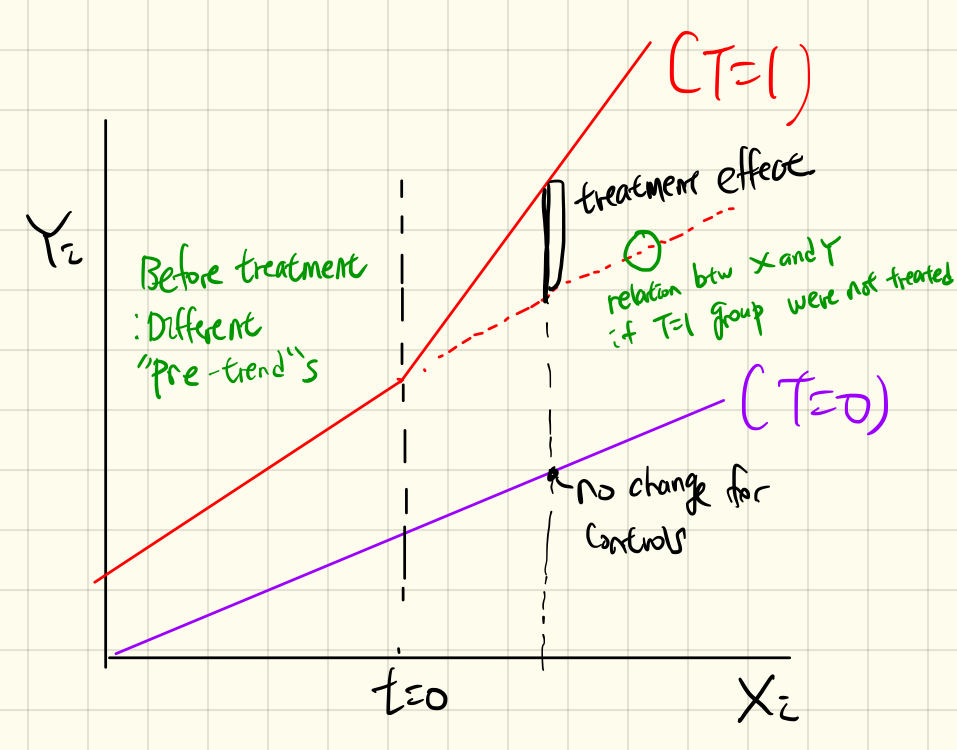
\includegraphics[width=\textwidth]{fig1_1.png}
\caption{No change in control group}
\end{subfigure}
\begin{subfigure}[b]{.4\textwidth}
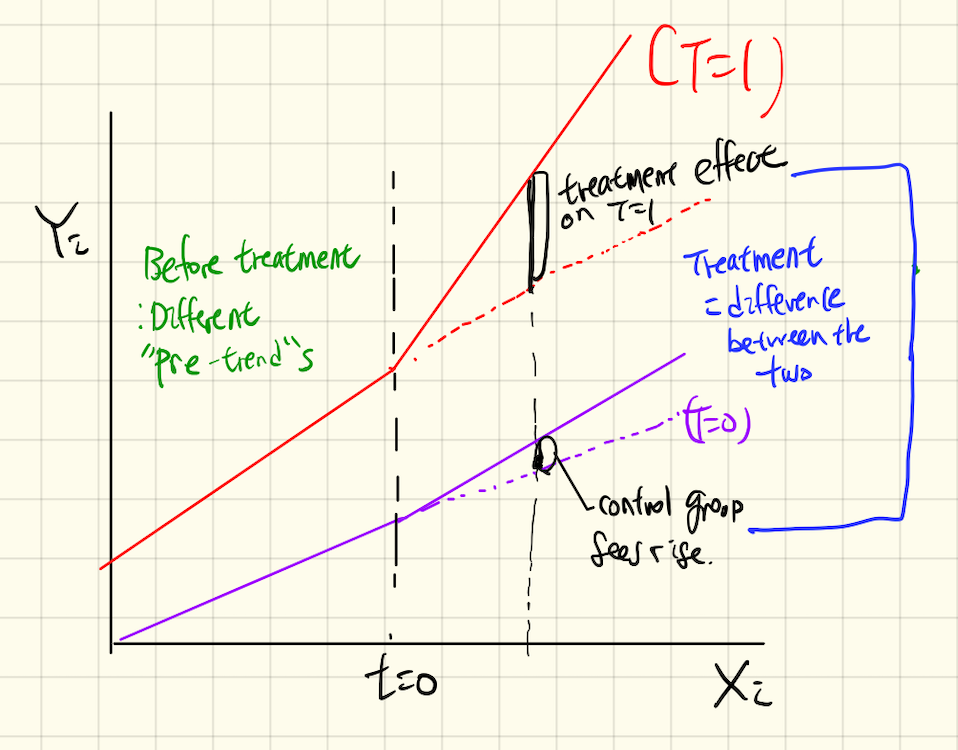
\includegraphics[width=\textwidth]{fig1_2.png}
\caption{Some change in control group}
\end{subfigure}
\end{figure}
In words, the treatment effect measured by the DD estimator is the treatment effect on treated groups \textit{on top of} effect on control groups. 
\par\medskip
\textbf{Regression discontinuity} design (or RD) applies to the case where the treatment status depends on whether individual $i$ has passed a threshold. Suppose that there is a variable $T_i$, like a test score, for instance. Let's assume that there exists a program for gifted students that only accept those whose test score is higher than 90. In this case, $X_i=1$ iff $T_i>90$ and $X_i=0$ if otherwise. In equation,
\[
Y_i  = \beta_0 + \beta_1X_i+u_i
\] 
and the following figure captures the treatment effect in an RD setup.
\begin{figure}[H]
\centering 
\caption{RD treatment effects}
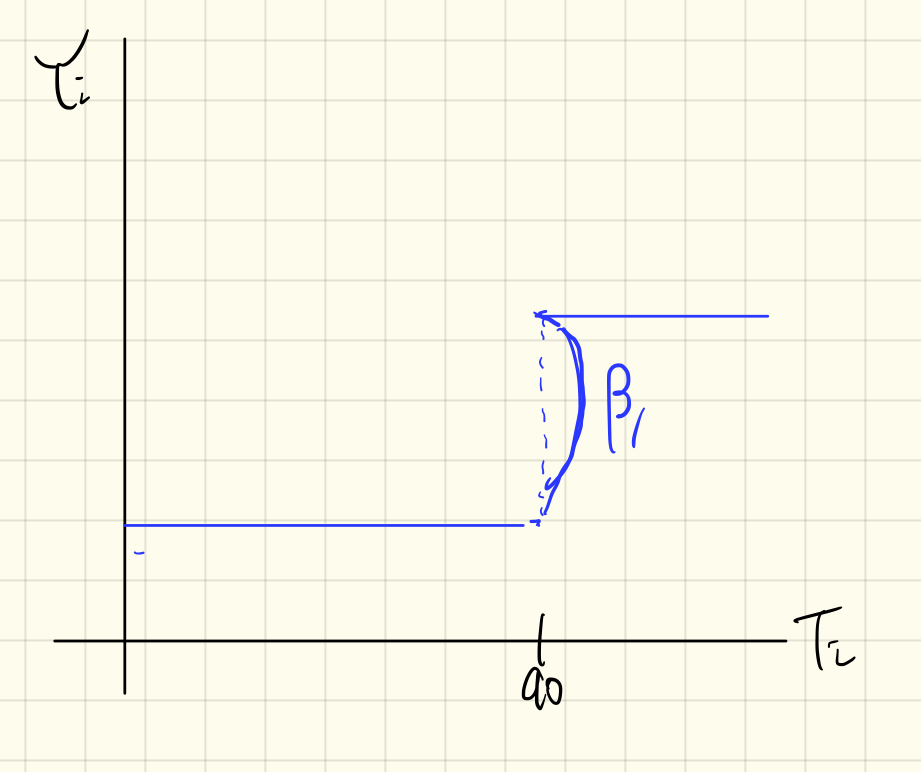
\includegraphics[width=0.4\textwidth]{fig2.png}
\end{figure}
For those not in the program, $E[Y_i|X_i=0]=\beta_0$ and $E[Y_i|X_i=1]=\beta_0+\beta_1$. This implies that if the direct effect of $T$ on $Y$ is continuous in the absence of the treatment, the effect of treatment should show up as a jump of size $\beta_1$ at the threshold value of $T_i$, 90 in our case. Similar to what we have in our figure

\par\medskip
To conduct RD rigorously, many things should be satisfied. Ideally, RD is most accurate in settings where subjects are not different in other traits (especially if we are including control variables $W_i$). In order to achieve this, we usually limit the subjects to those around certain bandwidth of the cutoff value of $T_i$. Therefore, it may induce a loss of sample issue. (This is actually an advanced topic)
\par\medskip
For now, I assumed that everyone whose $T_i>90$ is accepted. This is what is called \textbf{sharp RD}. However, this may not always be the case in reality. There might be exceptions - those whose test score are higher than 90 may not be part of the program and those whose score is under 90 might be part of the program. If this is the case and we carry out an RD here, we are conducting a \textbf{fuzzy RD}. The estimation in the case of fuzzy RD is tricky and quite advanced. So the takeaway here is that the accuracy of RD is susceptible to the compliance (of the program) issue. If the subjects are not fully complaint to the intentions of the program, accuracy of the RD is not fully guaranteed.  


